\documentclass[a4paper,12pt]{report}
\usepackage[T1]{fontenc}
\usepackage[utf8]{inputenc}
\usepackage[francais]{babel}
\usepackage[usenames,dvipsnames,svgnames,table]{xcolor}
\usepackage[colorlinks,linkcolor={blue!30!black},
                       citecolor={blue!50!black},
                        urlcolor={blue!80!black},
                        ]{hyperref}
\usepackage{titling} % Récupérer titre et auteur
\usepackage{enumerate} % Styles personnalisés d'énumération
\usepackage{amsmath,siunitx,array,url} % Symboles, etc
\usepackage{caption,subcaption,wrapfig,rotating,pdfpages} % Mise en page
\usepackage[perpage]{footmisc} % Numérotation par page des footnotes
\usepackage{epic,eepic,graphicx,tikz} % Drawings
\usepackage[top=2cm,left=2.5cm,right=2.5cm,bottom=2cm]{geometry} % Géométrie de la page, modifier selon le besoin
\setlength{\parskip}{0.4em} % Taille des interlignes entre paragraphes
\usepackage[babel=true,kerning=true]{microtype}

\addto{\captionsfrench}{\renewcommand{\abstractname}{Introduction}}
\pdfsuppresswarningpagegroup=1
\date{}
\title{Rapport de Projet de Fin d'Études : Caractérisation de pointes fibrées pour nano-pinces optiques et plasmoniques}
\author{Félix Piédallu}
\hypersetup{pdftex,
            pdfauthor=\theauthor,
            pdftitle=\thetitle}

\begin{document}
\nocite{*}
\pagenumbering{gobble}  % Pas de numérotation
\begin{titlepage}
    \vspace*{-10px}
    
\includegraphics[height=80px]{Images/logo_phelma.pdf}
    \vspace*{-80px}
\begin{flushright}
    \vspace*{-10px}
    
\includegraphics[height=80px]{Images/Logo_Neel.pdf}
\end{flushright}

\vspace*{1.5cm}
\begin{center}
\rule{\linewidth}{0.5mm}\\[0.4cm]
{\huge{\bfseries Rapport de Projet de Fin d'Études}\\[0.4cm]
Caractérisation de pointes fibrées pour nano-pinces optiques et plasmoniques\\[0.4cm]}
\rule{\linewidth}{0.5mm}\\[0.5cm]

\LARGE{\textsc{Félix Piédallu}}\\[0.7cm]
\large{\textsc{Filière PNS 2015-2016}}\\[2cm]

\Large{Au sein de l'équipe Nano-Optique et Forces}\\[1cm]

\Large{Sous la direction de Jochen \textsc{Fick}}\\[2cm]

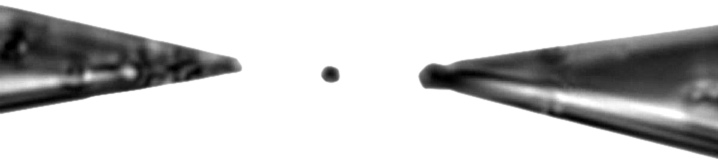
\includegraphics[width=\textwidth]{Images/Illustration.png}\\[1cm]


\end{center}
\end{titlepage}

\tableofcontents        % Table des matières avec liens, générée automatiquement.
\newpage
\listoffigures
\pagenumbering{arabic}  % Numérotation de retour !


\chapter*{Introduction} % Contexte du stage
\section*{Les pinces optiques}
Introduites en 1986 par A. Ashkin\cite{Ashkin}, les pinces optiques permettent de piéger et de manipuler, sans contact mécanique, des objets nanométriques. Cette particularité non destructive ni invasive les affirme comme un outil privilégié pour la manipulation et l'isolation de molécules et d'espèces biologiques.

Leur fonctionnement repose sur les forces d'interaction entre la matière et le rayonnement optique injecté par la pince. D'une part, la force de gradient attire les particules vers les maxima d'intensité lumineuse, permettant de les piéger au centre d'un faisceau, et proche de la source lumineuse. D'autre part, la force de diffusion pousse les particules dans le sens de propagation du faisceau. La conception d'une pince optique efficace et stable repose alors sur un bon équilibre entre ces deux forces.

Les pinces optiques classiques utilisent alors un faisceau laser gaussien fortement focalisé, afin de maximiser la force de gradient au point focal, et donc l'efficacité du piégeage. Mais depuis les années 2000, les pinces optiques fibrées semble une voie privilégiée pour le piégeage optique \cite{Taguchi,Taylor}. Elles ne nécessitent pas de matériel optique encombrant et peuvent être intégrées et alignées facilement.

De telles pinces optiques utilisent comme source de faisceau des fibres gravées en pointes afin d'obtenir un faisceau très concentré, et donc des gradients l'intensité lumineuse élevés.

\section*{Contexte du stage}
Le dispositif actuel de pince optique fibrée a été développé dans le cadre de la thèse de Jean-Baptiste Decombe\cite{Decombe}. Elle est composée de deux fibres optiques monomodes, gravées à une extrémité en pointe, ce qui permet d'obtenir un faisceau Gaussien de quelques microns de largeur.

Cette pince optique a permis un piégeage efficace de particules diélectriques sphériques, de tailles allant du micron à quelques 60nm de diamètre.

Le but de mon stage est alors de caractériser au mieux les pointes utilisées afin de connaître au mieux leur émission, spatialement et spectralement. Cela permettra notamment de connaître correctement les différents types de pointes et leurs applications possibles.

Dans une première partie, nous allons détailler l'ensemble du dispositif expérimental que j'ai utilisé durant mon stage, et le protocole d'élaboration des pointes fibrées. Ensuite, nous verrons les caractérisations en émission spatiales et spectrales que j'ai effectuées.

\chapter{L'expérience}

\section{La mise en place de l'expérience}
\subsection{Dérive des moteurs Mechonics}
Utilisation de deux fibres métallisées (Spot plus petit = meilleure précision).

On peut remarquer dans la figure \ref{mechonics_avant} que la fibre fixée sur les Mechonics se déplace jusqu'à 500 nm/minute. Cette dérive suit une loi exponentielle, on a alors supposé une relâche mécanique des supports, ou bien électrique au niveau du contrôleur: une mauvaise mise à la masse des moteurs pourrait entraîner une telle dérive.

Après mise à la masse des connecteurs des Mechonics, cette vitesse est tombée à 23 nm/minute selon Y et même 3nm/minute selon Z, comme on peut le voir sur la courbe \ref{mechonics_apres}.
\par


\begin{figure}[h] \centering
    \begin{subfigure}[b]{0.48\textwidth}
        \includegraphics[width=\textwidth]{{"Images/Derive_Mecho/Avant"}.png}
        \caption{Avant mise à la masse}
        \label{mechonics_avant}
    \end{subfigure}
    \begin{subfigure}[b]{0.48\textwidth}
        \includegraphics[width=\textwidth]{{"Images/Derive_Mecho/Apres"}.png}
        \caption{Après mise à la masse}
        \label{mechonics_apres}
    \end{subfigure}
    \caption{Déplacement des Mechonics avant mise à la masse}
\end{figure}


\section{Les appareils de mesure}
\section{L'élaboration des pointes \& des pointes métallisées}

\subsection{Images FIB}
L'excentricité de l'apex d'une pointe de petit axe $a$ et grand axe $b$ est définie par 
\[e=\frac{\sqrt{a^2-b^2}}{a}\]
\begin{figure}[h]\centering
    \begin{subfigure}[b]{0.35\textwidth}\label{l27fm5_meb}
        \includegraphics[width=\textwidth]{{"Images/Photos_Fibres/l27fm5_ronde_crop"}.png}
        \caption*{Apex circulaire ($e = 0,28$)}
    \end{subfigure}
    \begin{subfigure}[b]{0.35\textwidth}\label{l40fm3_meb}
        \includegraphics[width=\textwidth]{{"Images/Photos_Fibres/l40fm3_dims_crop"}.png}
        \caption*{Apex allongé ($e = 0,98$)}
    \end{subfigure}
    \caption{Clichés MEB de pointes coupées au FIB}
    \label{fib_ronde_allongee}
\end{figure}


\begin{figure}[h]\centering
    \begin{subfigure}[b]{0.25\textwidth}\label{l33fm2_meb_avant}
        \includegraphics[width=\textwidth]{{"Images/Photos_Fibres/l33fm2_avant_crop"}.jpg}
    \end{subfigure}
    \begin{subfigure}[b]{0.25\textwidth}\label{l33fm2_meb}
        \includegraphics[width=\textwidth]{{"Images/Photos_Fibres/l33fm2_apres_crop"}.jpg}
    \end{subfigure}
    \caption{Pointe métallisée avant et après découpe au FIB}
    \label{fib_avant_apres}
\end{figure}

\section{Couplage dans la fibre multimode}
Dummy text


\chapter{Caractérisation des pointes}
Nous allons détailler dans ce chapitre les différentes méthodes de caractérisation des pointes, afin de mettre en valeur les propriétés des différentes pointes qui ont été étudiées.

Dans un premier temps nous allons observer l'émission des pointes en fonction de la polarisation de la lumière injectée dans la fibre. \par

Ensuite, nous allons mesurer l'évolution de la transmission des pointes en fonction de la distance entre la pointe émettrice et la pointe de mesure. Ceci nous permettra de comprendre la structure du spot émis, et d'en conclure sur leur utilisabilité dans le cadre des nano-pinces optiques. \par

Enfin, nous allons étudier le spectre de transmission d'une telle pince, afin de mettre en valeur la transmission des différents éléments de la pince optique.

\section{Influence de la polarisation incidente sur l'émission}
Il avait été vu dans de précédentes études que la transmission des pointes métallisées dépendait fortement de la polarisation de la lumière incidente \cite{Decombe}. Notamment, cette dépendance doit se retrouver exclusivement pour des apex elliptiques.
Les modélisations qui avaient été effectuées peuvent être retrouvées dans la figure \ref{theorie_polar_metal}.
\begin{figure}[h]\centering
    \includegraphics[width=0.15\textwidth]{{"Images_pasmoi/Polar_0"}.png}\hspace*{5mm}
    \includegraphics[width=0.15\textwidth]{{"Images_pasmoi/Polar_32"}.png}\hspace*{5mm}
    \includegraphics[width=0.15\textwidth]{{"Images_pasmoi/Polar_90"}.png}
    \caption{Intensité calculée avec trois polarisations incidentes caractéristiques \cite{Decombe}}
    \label{theorie_polar_metal}
\end{figure}

\subsection{Pointes sans métal}
Nous avons d'abord décidé de vérifier que les pointes non métallisées n'ont pas de dépendance en polarisation.

La figure \ref{var_lambda_nues} présente les profils d'émission d'une pointe non métallisée à deux polarisations incidentes orthogonales. On constate facilement que la polarisation de la lumière incidente n'a pas d'impact sur l'émission: seule une petite variation d'intensité traduit les irrégularités des pointes utilisées.
\begin{figure}
    \begin{center}
        \includegraphics[width=.5\textwidth]{Images/Photos_Fibres/Camera/Pointes_nues_air_crop.png}
        \caption{Photo au microscope de deux pointes non métallisées, une en mauvais état (gauche) et en bon état (droite)}
        \label{pointes_nues_photo}
    \end{center}
\end{figure}

\begin{figure}[h]\centering
    \begin{subfigure}[b]{0.15\textwidth}
        \includegraphics[width=\textwidth]{{"Images/Var_Lambda/Nues_2/0deg"}.png}
        \caption{$\theta$ = 0\si{\degree}}
    \end{subfigure}
    \begin{subfigure}[b]{0.15\textwidth}
        \includegraphics[width=\textwidth]{{"Images/Var_Lambda/Nues_2/45deg"}.png}
        \caption{$\theta$ = 90\si{\degree}}
    \end{subfigure}
    \caption{Influence de la polarisation sur la transmission de pointes non métallisées}
    \label{var_lambda_nues}
\end{figure}

Ce résultat nous permet notamment de nous assurer de la validité des prochaines mesures: (TODO trouver une formulation)

\subsection{Pointes métallisées}
Nous avons donc ensuite observé l'effet de la polarisation de la lumière incidente sur l'émission d'une pointe métallisée. Nous avons utilisé une fibre non métallisée pour mesurer le profil d'émission d'une pointe métallisée, afin de ne mesurer qu'un effet dû à cette pointe métallisée.

La figure \ref{var_lambda_metal} présente les résultats obtenus avec une pointe très allongée (fig. \ref{pointe_metal_var_lambda}), dans l'air, avec une distance entre les pointes de l'ordre du micron.

\begin{figure}[h]\centering
    \includegraphics[width=0.2\textwidth]{{"Images/Photos_Fibres/l40fm3_dims_crop_2"}.png}
    \caption{Pointe allongée (excentricité $= 0,98$)}\vspace*{5mm}
    \label{pointe_metal_var_lambda}

    \begin{subfigure}[b]{0.136\textwidth}
        \includegraphics[width=\textwidth]{{"Images/Var_Lambda/Metal_2/32d"}.png}
        \caption*{$\theta$ = 0\si{\degree}}
    \end{subfigure}
    \begin{subfigure}[b]{0.136\textwidth}
        \includegraphics[width=\textwidth]{{"Images/Var_Lambda/Metal_2/47d"}.png}
        \caption*{$\theta$ = 30\si{\degree}}
    \end{subfigure}
    \begin{subfigure}[b]{0.136\textwidth}
        \includegraphics[width=\textwidth]{{"Images/Var_Lambda/Metal_2/62d"}.png}
        \caption*{$\theta$ = 60\si{\degree}}
    \end{subfigure}
    \begin{subfigure}[b]{0.136\textwidth}
        \includegraphics[width=\textwidth]{{"Images/Var_Lambda/Metal_2/77d_2"}.png}
        \caption*{$\theta$ = 90\si{\degree}}
    \end{subfigure}
    \begin{subfigure}[b]{0.136\textwidth}
        \includegraphics[width=\textwidth]{{"Images/Var_Lambda/Metal_2/92d"}.png}
        \caption*{$\theta$ = 120\si{\degree}}
    \end{subfigure}
    \begin{subfigure}[b]{0.136\textwidth}
        \includegraphics[width=\textwidth]{{"Images/Var_Lambda/Metal_2/107d"}.png}
        \caption*{$\theta$ = 150\si{\degree}}
    \end{subfigure}
    \begin{subfigure}[b]{0.136\textwidth}
        \includegraphics[width=\textwidth]{{"Images/Var_Lambda/Metal_2/122d_3"}.png}
        \caption*{$\theta$ = 180\si{\degree}}
    \end{subfigure}
    \caption{Profils d'émission en fonction de la polarisation incidente}
    \label{var_lambda_metal}
\end{figure}

On peut tout d'abord noter que les spots semblent beaucoup plus larges ($\sim 4\mu m$) que l'apex de la pointe métallisée, qui est de l'ordre de 200nm. Nous mesurons en effet, comme nous l'avons vu dans la première partie (TODO), la convolution entre la fibre émettrice et réceptrice ; La fibre réceptrice, non métallisée, a une grande ouverture optique, ce qui donne de telles mesures.

Enfin, on remarque bien une dépendance en polarisation telle qu'on l'attendait: pour $\theta = 0\si{\degree}$, il apparaît deux spots assez éloignés, la lumière incidente est alors polarisée selon le petit axe de la pointe métallisée ; tandis que pour  $\theta = 90\si{\degree}$, on ne peut distinguer qu'un seul lobe: on ne distingue pas les deux spots prévus par la simulation.

Ces mesures nous permettent notamment de conclure que le grand axe de notre pointe métallisée est orienté horizontalement selon les profils d'émission.

%TODO mettre ça dans la première partie %De telles mesures ont donc été effectuées, en faisant varier la polarisation injectée grâce à un polariseur (qui permet de filtrer une seule polarisation) et une lame $\lambda/2$ (qui permet de faire varier cette polarisation).

%TODO: utiliser 2 pointes applaties ? Déjà fait, p. 30… Pas très concluant.
%On peut alors observer dans les figures \ref{var_lambda_200nm} et \ref{var_lambda_3um} les spectres selon la polarisation. La pointe métalisée est relativement ronde, ce qui se traduit par une assez faible dépendance en polarisation. On observe tout de fois un déplacement du spot principal d'émission entre $\theta/2 = 0^o$ et $\theta/2 = 45^o$.
% \begin{figure}\centering
%         \includegraphics[width=0.3\textwidth]{{"Images/Photos_Fibres/l27fm5_ronde"}.png}
%         \caption{Pointe métallisée presque circulaire (peu de dépendance en polarisation)}
%         \label{l27fm5_photo}
% \end{figure}



\subsection{Pointes de Bessel}
Nous avons effectué les mêmes mesures avec une pointe de Bessel. Nous attendons le même résultat que pour les fibres non métallisées: pas, ou très peu, de dépendance en polarisation incidente.

TODO rapide explication théorique ?

Nous avons alors utilisé une fibre non métallisée pour étudier l'émission, dans l'air, d'une pointe de Bessel. On constate bien sur la figure \ref{var_lambda_bessel} que la polarisation n'a pas d'incidence sur l'émission mesurée, cela confirme nos attentes.

\begin{figure}[h]\centering
    \includegraphics[width=0.4\textwidth]{{"Images/Photos_Fibres/Camera/Bessel_1"}.png}
    \caption{Photo au microscope d'une pointe de Bessel}\vspace*{5mm}
    \label{pointe_bessel_var_lambda}

    \begin{subfigure}[b]{0.136\textwidth}
        \includegraphics[width=\textwidth]{{"Images/Bessel/VarLambda/0d"}.png}
        \caption*{$\theta$ = 0\si{\degree}}
    \end{subfigure}
    \begin{subfigure}[b]{0.136\textwidth}
        \includegraphics[width=\textwidth]{{"Images/Bessel/VarLambda/15d"}.png}
        \caption*{$\theta$ = 30\si{\degree}}
    \end{subfigure}
    \begin{subfigure}[b]{0.136\textwidth}
        \includegraphics[width=\textwidth]{{"Images/Bessel/VarLambda/30d"}.png}
        \caption*{$\theta$ = 60\si{\degree}}
    \end{subfigure}
    \begin{subfigure}[b]{0.136\textwidth}
        \includegraphics[width=\textwidth]{{"Images/Bessel/VarLambda/45d"}.png}
        \caption*{$\theta$ = 90\si{\degree}}
    \end{subfigure}
    \begin{subfigure}[b]{0.136\textwidth}
        \includegraphics[width=\textwidth]{{"Images/Bessel/VarLambda/60d"}.png}
        \caption*{$\theta$ = 120\si{\degree}}
    \end{subfigure}
    \begin{subfigure}[b]{0.136\textwidth}
        \includegraphics[width=\textwidth]{{"Images/Bessel/VarLambda/75d"}.png}
        \caption*{$\theta$ = 150\si{\degree}}
    \end{subfigure}
    \begin{subfigure}[b]{0.136\textwidth}
        \includegraphics[width=\textwidth]{{"Images/Bessel/VarLambda/90d"}.png}
        \caption*{$\theta$ = 180\si{\degree}}
    \end{subfigure}
    \caption{Profils d'émission en fonction de la polarisation incidente}
    \label{var_lambda_bessel}
\end{figure}


\section{Variation de la distance}
Une caractéristique importante des pointes est l'évolution du spot d'émission en fonction de la distance. En effet, cela détermine directement les performance du piégeage optique en fonction de la distance entre les pointes qui forment la pince optique.

Pour cela, nous mesurons les profils d'émission des pointes, en éloignant la pointe de mesure de la pointe émettrice. Nous obtenons alors des spots gaussiens, dont la largeur évolue en fonction de la distance.

Dans un premier temps, nous avons caractérisé les pointes dans l'air, puis dans l'eau afin de se rapprocher des conditions expérimentales des pinces optiques.

\subsection{Pointes sans métal}
On peut facilement reconnaître des fibres de bonne et mauvaise qualité: une pointe correcte présente un spot d'émission gaussien, quelle que soit la distance de mesure. La figure \ref{fibre_ok_scan} présente des exemples de scans caractéristiques.

\begin{figure}[h]\centering
    \begin{subfigure}[b]{0.136\textwidth}
        \includegraphics[width=\textwidth]{{"Images/Vrac/Nue_OK_1"}.png}
        \caption{}
    \end{subfigure}
    \begin{subfigure}[b]{0.136\textwidth}
        \includegraphics[width=\textwidth]{{"Images/Vrac/Nue_Pasok"}.png}
        \caption{}
    \end{subfigure}
    \caption{Exemples de profils de transmission caractéristiques pour une bonne (a) et une mauvaise (b) pointes}
    \label{fibre_ok_scan}
\end{figure}


\begin{figure}[h]\centering
TODO inclure les scans + une courbe d'évolution dans l'air et dans l'eau
    \caption{Profils d'émission dans l'air (-) et dans l'eau (-) et évolution du waist avec la distance ()}
    \label{nues_distance}
\end{figure}

La largeur des spots évolue linéairement avec la distance dans l'air et dans l'eau, avec une largeur au contact autour de $nm$ dans les deux milieux.
On obtient l'angle d'émission de la pointe à partir de la pente du waist: $\theta_{\text{émission}} = \arctan(\text{pente}) $, et l'ouverture numérique de la pointe est définie par:
\[
    N.A = n\sin(\frac{\theta}{2})
\]
où $\theta$ est l'angle total du cône d'émission.

Dans l'air, on trouve un angle d'émission de $18\si{\degree}$, qui donne une ouverture numérique de 0,16.

Dans l'eau, le saut d'indice entre la fibre (n=1,45) et l'eau (1,33) beaucoup étant moins important qu'avec l'air (n=1), le faisceau diverge beaucoup moins: on obtient un angle d'émission de $8\si{\degree}$ et une ouverture numérique de 0,09.

Enfin, l'amplitude de l'intensité lumineuse transmise évolue selon $\dfrac{1}{\sqrt{\text{distance}}}$: en effet le flux total transmis entre les deux pointes reste constant tandis que la surface de transmission évolue quadratiquement.

Cette intensité est trois fois plus importante dans l'eau que dans l'air: cela implique un facteur $\sqrt{3}$ en puissance.


\subsection{Pointes métalliques}
Nous avons alors fait la même étude pour des pointes métalliques. Ici nous avons pris une pointe la plus circulaire possible, pour limiter l'impact de la polarisation incidente sur l'émission.

La figure \ref{emission_metal_distance} présente les scans effectués dans l'air à très faible distance ($d=50nm$) et à distance plus élevée ($d=1\mu m$) ainsi que la courbe d'évolution de la largeur du spot. 

On remarque tout d'abord que le spot, à faible distance, est de forme elliptique : on retrouve la forme de l'apex de la pointe métallique utilisée. En s'éloignant de la pointe, le spot devient progressivement circulaire.

\begin{figure}[h]\centering
    \begin{subfigure}[c]{0.156\textwidth}
        \includegraphics[width=\textwidth]{{"Images/Metal/VarDistance/26"}.png}
        \caption*{$d = 50nm$}
    \end{subfigure}
    \begin{subfigure}[c]{0.5\textwidth}
        \includegraphics[width=\textwidth]{{"Images/Metal/VarDistance/VarDistance"}.png}
        \caption*{Évolution du waist avec la distance}
    \end{subfigure}
    \begin{subfigure}[c]{0.156\textwidth}
        \includegraphics[width=\textwidth]{{"Images/Metal/VarDistance/25"}.png}
        \caption*{$d = 1\mu m$}
    \end{subfigure}
    \caption{Émission d'une pointe métallique en fonction de la distance entre les pointes}
    \label{emission_metal_distance}
\end{figure}

Enfin, nous avons à faible distance une évolution quadratique, puis une évolution linéaire au-delà de 800nm.


\subsection{Pointes de Bessel}
Enfin, nous avons étudié l'évolution de l'émission d'une pointe de Bessel en fonction de la distance.

Compte tenu de la structure du faisceau de Bessel (ref chapitre 1), nous attendons une divergence très lente du spot avec la distance. C'est pourquoi, contrairement aux pointes métalliques pour lequelles nous n'avons pas dépassé quelques microns de distance de mesure, nous sommes allés jusqu'à $220\mu m$ pour les pointes de Bessel.

\begin{figure}[h]\centering
    \begin{subfigure}[b]{0.136\textwidth}
        \includegraphics[width=\textwidth]{{"Images/Bessel/VarDistance/fS2_d=4.9"}.png}
        \caption*{d=5$\mu$m}
    \end{subfigure}
    \begin{subfigure}[b]{0.136\textwidth}
        \includegraphics[width=\textwidth]{{"Images/Bessel/VarDistance/fS2_d=62"}.png}
        \caption*{d=60$\mu$m}
    \end{subfigure}
    \begin{subfigure}[b]{0.136\textwidth}
        \includegraphics[width=\textwidth]{{"Images/Bessel/VarDistance/fS2_d=101"}.png}
        \caption*{d=100$\mu$m}
    \end{subfigure}
    \begin{subfigure}[b]{0.136\textwidth}
        \includegraphics[width=\textwidth]{{"Images/Bessel/VarDistance/fS2_d=150"}.png}
        \caption*{d=150$\mu$m}
    \end{subfigure}
    \begin{subfigure}[b]{0.136\textwidth}
        \includegraphics[width=\textwidth]{{"Images/Bessel/VarDistance/fS2_d=197"}.png}
        \caption*{d=200$\mu$m}
    \end{subfigure}\\
    \includegraphics[width=0.5\textwidth]{{"Images/Bessel/VarDistance/waist2"}.png}
    TODO épurer la figure
    \caption{Variation de l'émission d'une pointe de Bessel en fonction de la distance}
    \label{var_distance_bessel}
\end{figure}

On constate en effet sur la figure \ref{var_distance_bessel} que le spot évolue linéairement très peu sur $200\mu m$. On obtient un angle d'ouverture autour de $0.47\si{\degree}$. Cela promet un piégeage très efficace sur de grandes distances.

Paradoxalement, l'intensité transmise dans le spot n'est pas constante : elle évolue selon $\dfrac{1}{\sqrt{\text{distance}}}$ comme pour des pointes classiques.TODO explication

En effet, pour obtenir une intensité constante, il faudrait que les plans d'onde formant le faisceau de Bessel soient infinis, ce qui est en pratique impossible.


\subsubsection*{Franges d'émission des pointes de Bessel}
Une autre façon d'étudier est d'observer les franges du faisceau de Bessel. Or l'amplitude de ces franges est extrêmement faible face à celle du spot central. Pour cela, nous imposons alors à notre mesure d'être saturée au niveau du spot, pour observer facilement les franges. La figure \ref{franges_bessel} présente de telles mesures, et nous pouvons voir le déplacement des franges

Un outil numérique nous permet enfin de mesurer le rayon des franges. La figure \ref{franges_bessel_courbe} présente l'évolution du rayon d'une des franges observables.


\begin{figure}[h]\centering
    \begin{subfigure}[b]{0.156\textwidth}
        \includegraphics[width=\textwidth]{{"Images/Bessel/Franges/d=5"}.png}
        \caption*{5$\mu$m}
    \end{subfigure}
    \begin{subfigure}[b]{0.156\textwidth}
        \includegraphics[width=\textwidth]{{"Images/Bessel/Franges/d=14"}.png}
        \caption*{14$\mu$m}
    \end{subfigure}
    \begin{subfigure}[b]{0.156\textwidth}
        \includegraphics[width=\textwidth]{{"Images/Bessel/Franges/d=20"}.png}
        \caption*{20$\mu$m}
    \end{subfigure}
    \begin{subfigure}[b]{0.156\textwidth}
        \includegraphics[width=\textwidth]{{"Images/Bessel/Franges/d=35"}.png}
        \caption*{30$\mu$m}
    \end{subfigure}
    \begin{subfigure}[b]{0.156\textwidth}
        \includegraphics[width=\textwidth]{{"Images/Bessel/Franges/d=40"}.png}
        \caption*{40$\mu$m}
    \end{subfigure}
    \begin{subfigure}[b]{0.156\textwidth}
        \includegraphics[width=\textwidth]{{"Images/Bessel/Franges/d=50"}.png}
        \caption*{50$\mu$m}
    \end{subfigure}
    \caption{Franges de Bessel en fonction de la distance}
    \label{franges_bessel}
\end{figure}

\begin{figure}[h]
    \begin{center}
        \includegraphics[width=0.7\textwidth]{{"Images/Bessel/Franges/Franges"}.png}
        \caption{Rayon des franges de Bessel en fonction de la distance}
        \label{franges_bessel_courbe}
    \end{center}
\end{figure}

La frange se déplace alors selon un angle de $8.5\mu m$, ce qui est beaucoup plus grand que l'angle de divergence du spot central.

\newpage
\section{Transmission en spectre}
Nous avons jusqu'ici étudié le profil spatial d'émission des pointes, pour les pointes non métallisées, métallisées et les pointes de Bessel.

Un autre axe d'étude du dispositif consiste à mesurer la transmission des pointes. Dans cette partie, nous nous intéresserons donc aux mesures en émission et transmission des différents types de pointes.


\subsection{Normalisation}
Dans un premier temps, il s'agit de "faire le blanc" en éliminant les contributions au spectre de la lumière blanche, des fibres et des connecteurs de fibres CamSplice.

La figure \ref{normalisation_transmission} présente ces résultats. Les courbes de gauche représentent les intensités mesurées avec la lampe blanche dirigée vers le spectromètre, puis lorsqu'on les connecte avec la fibre SM600, et enfin on connecte la fibre S630-HP entre deux fibres SM600.

Cette dernière configuration est, à l'exception des pointes elles-mêmes, équivalente à la configuration que nous utilisons pour mesurer la transmission des pointes. Elle nous servira donc de normalisation pour nos mesures suivantes.


\begin{figure}[h]\centering
    \begin{subfigure}[c]{0.7\textwidth}
        \includegraphics[width=\textwidth]{{"Images/Spectro/blancspectres"}.pdf}
    \end{subfigure}\\
    \begin{subfigure}[c]{0.4\textwidth}
        \includegraphics[width=\textwidth]{{"Images/Spectro/SpectresNormalisation"}.png}
    \end{subfigure}
    \begin{subfigure}[c]{0.4\textwidth}
        \includegraphics[width=\textwidth]{{"Images/Spectro/SpectresNormalisation-Transmission"}.png}
    \end{subfigure}
    \caption{Courbes de normalisation en intensité et en transmission}
    \label{normalisation_transmission}
\end{figure}

Ces mesures nous permettent aussi de constater qu'entre 600nm et 850nm, la transmission de notre dispositif reste stable.


\subsection{Caractérisation en spectre des pointes}
Nous avons donc effectué des mesures de transmission pour deux fibres non métallisées, puis pour une fibre métallisée émettant vers une fibre non métallisée. Pour chaque fibre, nous avons mesuré la transmission dans l'air et dans l'eau.

Nous nous attendons à 



\begin{figure}[h]
    \begin{center}
        \includegraphics[width=0.47\textwidth]{{"Images/Spectro/Intensite_toutes"}.png}
        \includegraphics[width=0.47\textwidth]{{"Images/Spectro/Transmission_toutes"}.png}
        \caption{Transmission des pointes nues et métallisées, dans l'eau et dans l'air}
    \end{center}
    \label{pointes_transmission}
\end{figure}



\chapter*{Bilan}
\addcontentsline{toc}{chapter}{Bilan}
%\input{}



\bibliographystyle{unsrt}
\bibliography{bibliographie}
\newpage
\appendix
\phantomsection
\addcontentsline{toc}{part}{Annexes}

\vspace*{8cm}
\begin{center}
\rule{\linewidth}{0.5mm}\\[0.7cm]
{\huge{\bfseries Annexes}}\\[0.4cm]
\rule{\linewidth}{0.5mm}\\[0.5cm]


\end{center}
%\newpage
%\phantomsection
%\addcontentsline{toc}{chapter}{Guide de câblage du cryostat}
%\includepdf[pages={-}]{../guide.pdf}

\newpage
%\input{9.Abstract}

\end{document}
